\subsection{Activity}%
\label{sec:activity}
An Android activity  is a view that allows user interaction. Generally, an app can have multiple activities but always starts with the main activity.
Each activity can start another to perform various tasks.
%
\subsubsection{Activity Lifecycle}%
\label{sec:activity_lifecycle}
The activities in the system are managed as activity stacks. The activities are organized in a stack, the back stack, in the order by which they were opened, meaning that when a new activity is started it is placed onto the top of the stack. The prior activity won't come into the foreground unless the current activity exits, e.g., when the user presses a back, home or similar return button.
%
Usually, the lifecycle of an android activity has this four key stages:
\begin{itemize}%
\item \textbf {Created}: In this stage the activity is beaing created.
\item \textbf {Resumed}:The activity is in the foreground thus now visible.
\item \textbf {Paused}: Another activity is in foreground but this one is still visible.
\item \textbf {Stopped}: The activity is running in the background and is no longer visible.
\end{itemize}
%
To control this lifecycle, one needs to implement the callback methods that refer to each specific stage by overwriting the pre-existing ones. The lifecycle of an activity is depicted in Fig.~\ref{fig:activity_lifecycle}.
%
\begin{figure}[!ht]
\centering
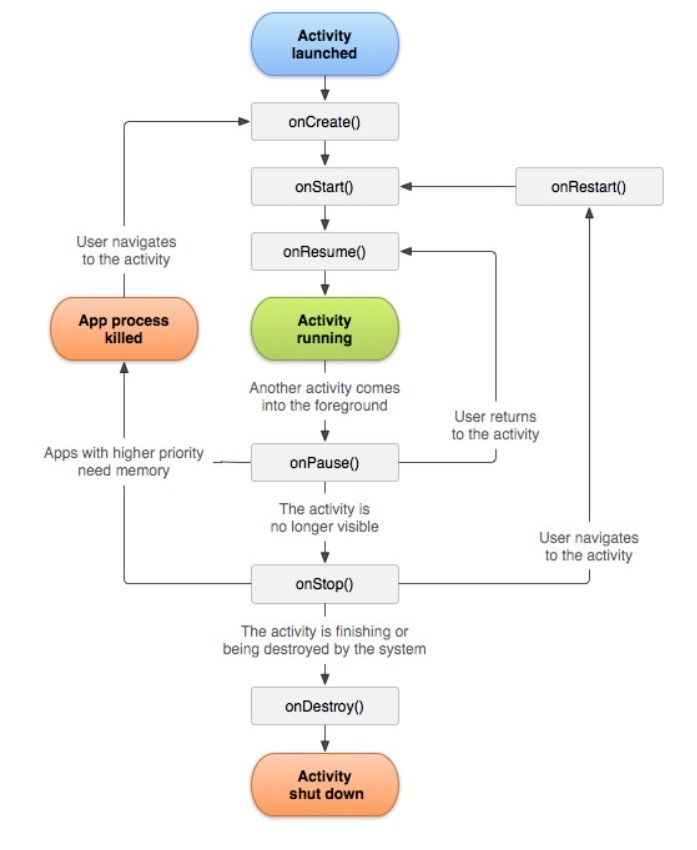
\includegraphics[width=0.8\textwidth]{img/activity_lifecycle.png}
\caption{\label{fig:activity_lifecycle}Android activity lifecycle
view }
\end{figure}
%%% Local Variables:
%%% mode: latex
%%% TeX-master: "../../../dissertation"
%%% End:
